\section{Results}

\subsection{E1: Orthogonality Validation}

\begin{table}[h]
\centering
\begin{tabular}{ll}
\toprule
\textbf{Metric} & \textbf{Value} \\
\midrule
Pearson $r$ & $-0.026$ \\
$p$-value & $0.250$ \\
\bottomrule
\end{tabular}
\caption{Orthogonality validation results.}
\end{table}

\textbf{Gate: PASSED.} The collaboration score is orthogonal to preference labels.

\subsection{E2: Training Stability}

\begin{table}[h]
\centering
\begin{tabular}{llll}
\toprule
\textbf{Step} & \textbf{DPO Loss} & \textbf{Agency Loss} & \textbf{Total Loss} \\
\midrule
100 & 0.679 & 0.500 & 0.929 \\
200 & 0.664 & 0.508 & 0.918 \\
\bottomrule
\end{tabular}
\caption{Training stability metrics.}
\end{table}

\textbf{Gate: PASSED.} BiDPO training is stable (loss decreases, zero NaN/Inf).

\subsection{E3: Generation Transfer (Negative Result)}

\begin{table}[h]
\centering
\begin{tabular}{llll}
\toprule
\textbf{Metric} & \textbf{DPO} & \textbf{BiDPO} & \textbf{Difference} \\
\midrule
Mean Score & 0.3728 & 0.3782 & +0.54\% \\
$p$-value (one-sided) & --- & --- & 0.247 \\
Cohen's $d$ & --- & --- & 0.016 \\
\bottomrule
\end{tabular}
\caption{Generation transfer results.}
\end{table}

\textbf{Gate: FAILED.} BiDPO shows marginal improvement but fails statistical significance.

\begin{figure}[h]
\centering
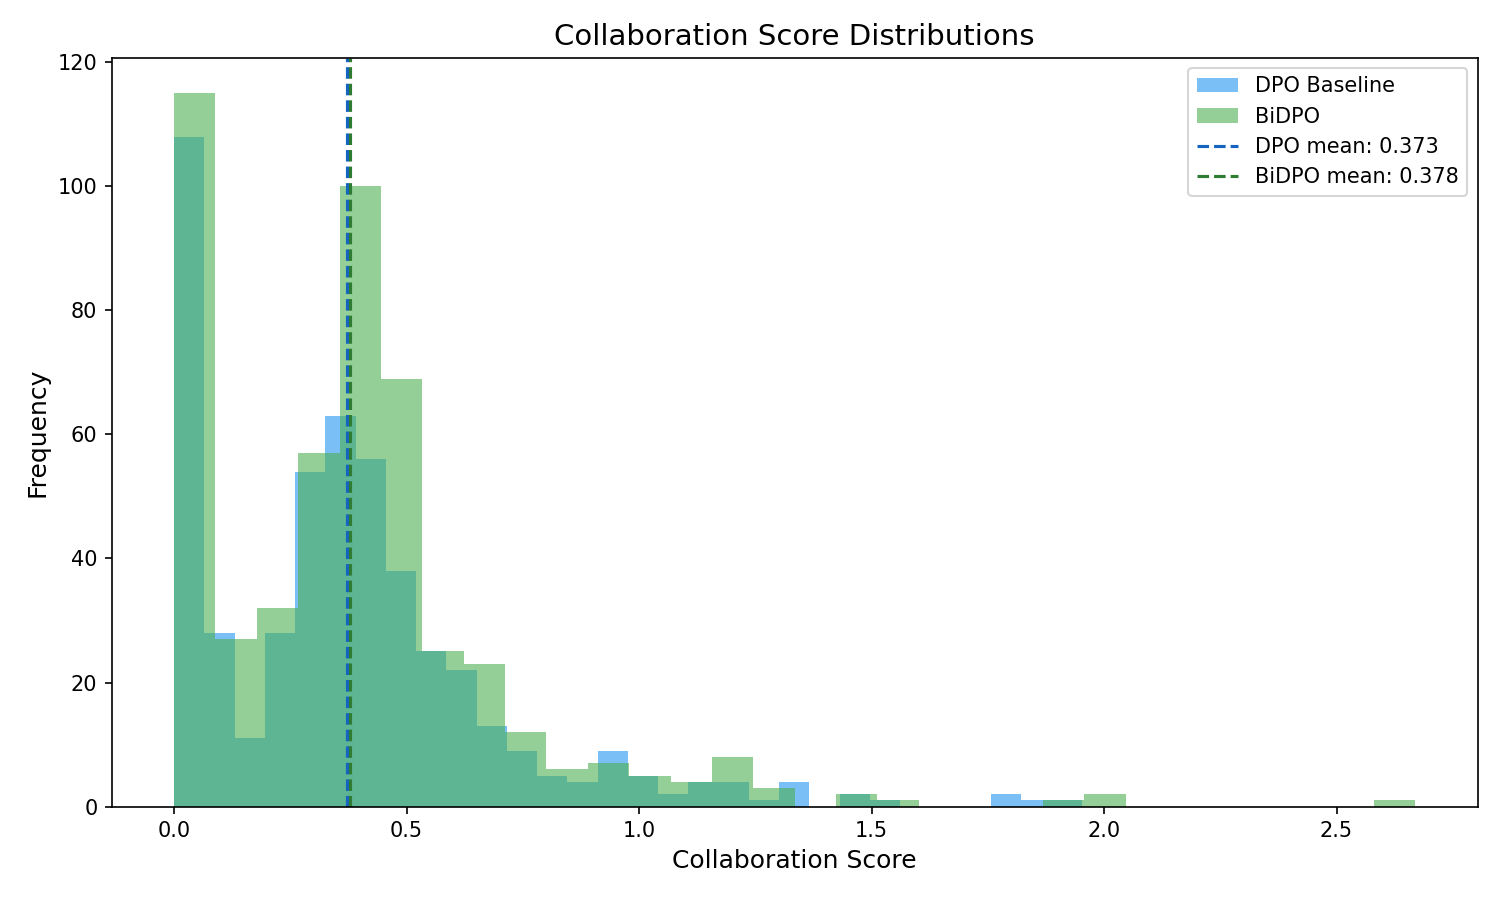
\includegraphics[width=0.8\textwidth]{figures/score_distributions.png}
\caption{Score distributions showing near-identical spreads for BiDPO and DPO.}
\label{fig:score_distributions}
\end{figure}

\subsection{Summary}

\begin{table}[h]
\centering
\begin{tabular}{lll}
\toprule
\textbf{Experiment} & \textbf{Gate} & \textbf{Result} \\
\midrule
E1: Orthogonality & MUST\_WORK & \textbf{PASSED} \\
E2: Training Stability & MUST\_WORK & \textbf{PASSED} \\
E3: Generation Transfer & SHOULD\_WORK & \textbf{FAILED} \\
\bottomrule
\end{tabular}
\caption{Experiment summary.}
\end{table}
